\section{Contexto Geográfico}

De acordo com dados da \citeaa{WikiPediaBrasilia20200518} A cidade começou a ser planejada e desenvolvida em 1956 por Lúcio Costa, pelo também arquiteto Oscar Niemeyer e pelo engenheiro estrutural Joaquim Cardozo. Inaugurada em 21 de abril de 1960, pelo então presidente Juscelino Kubitschek, Brasília tornou-se formalmente a terceira capital do Brasil, após Salvador e Rio de Janeiro. Vista de cima, a principal área da cidade é descrita frequentemente como tendo o formato de um avião, mas a proposta inicial de Lúcio Costa era de que se assemelhasse ao sinal da cruz, e um dos eixos foi depois arqueado para se adaptar ao relevo da região.\\

O ritmo de crescimento populacional na primeira década foi de 14,4\% ao ano, com um aumento populacional de 285\%. Na década de 1970, o crescimento médio anual foi de 8,1\%, com um incremento total de 115,52\%. A população total do Distrito Federal, que não deveria ultrapassar 500 000 habitantes em 2000, atingiu esta cota no início da década de 1970, e, entre 1980 e 1991, a população expandiu em mais 32,8\%. O Plano Piloto, que, na inauguração, concentrava 48\% da população do Distrito Federal, gradativamente perdeu importância relativa, chegando a 13,26\% em 1991, passando o predomínio para as cidades-satélite.


A população brasiliense é formada por migrantes de todas as regiões brasileiras, sobretudo do Nordeste e do Sudeste, além de estrangeiros que trabalham nas embaixadas espalhadas pela capital. Dados de 2010 apontavam que quase metade da população não nasceu ali, sendo que 1 380 873 (53,73\%) eram brasilienses e 1 189 287 (46,27\%) de outros locais (incluindo 8 577 estrangeiros, ou 0,33\% da população), principalmente de Goiás, Minas Gerais e Bahia, conforme o quadro abaixo da \citeaa{CODEPLANSEPLAN2013}.

\begin{figure}
    \centering
    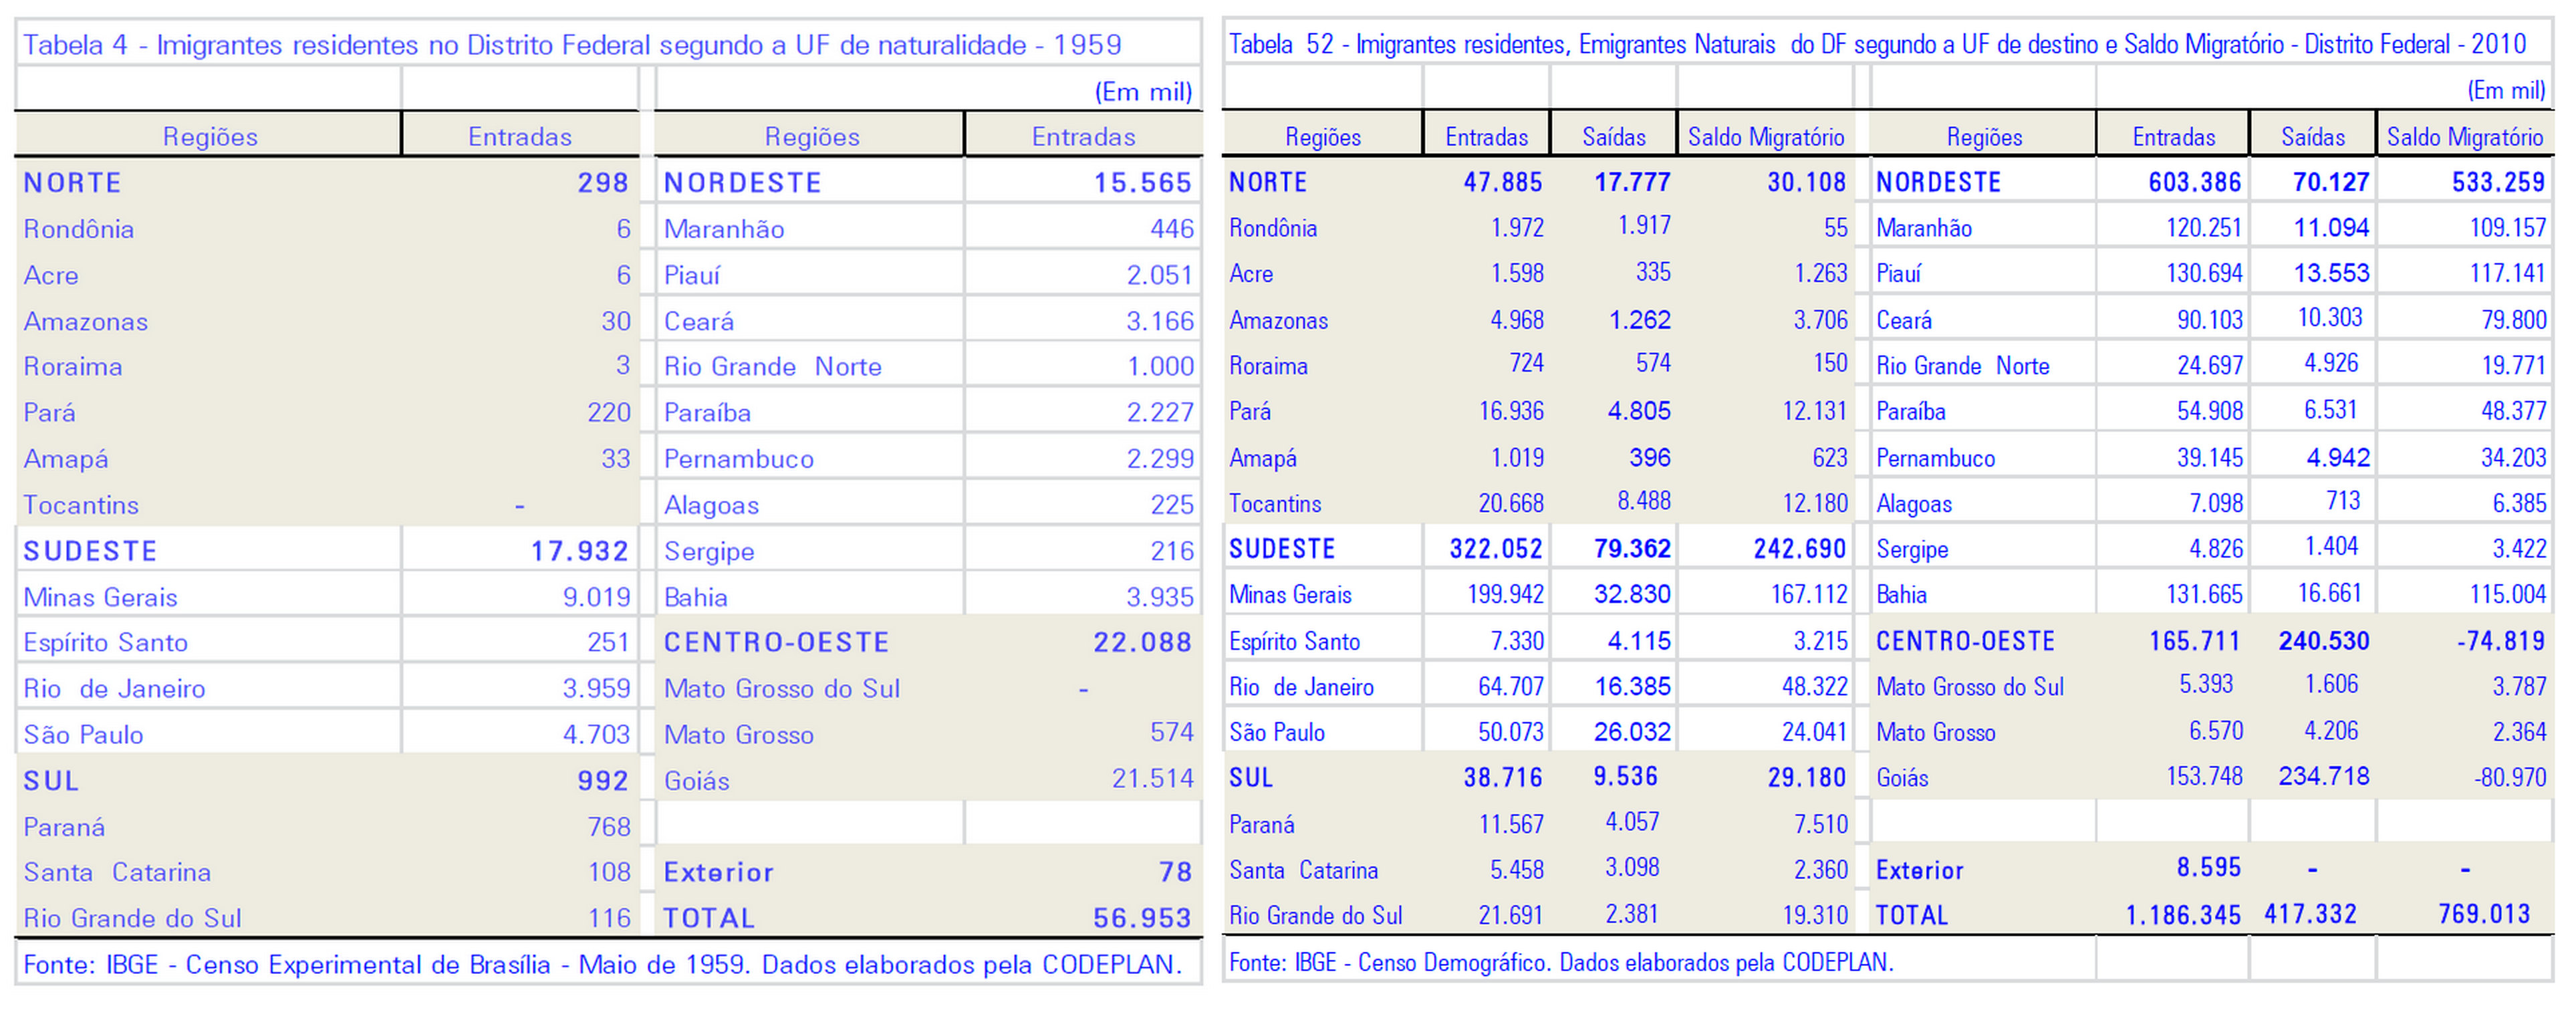
\includegraphics[width=0.95\linewidth]{fig/migrantes-1959-2010}
    \caption[Quadro comparativo de migrantes em brasília]{}
    \label{fig:migrantes-1959-2010}
\end{figure}


Em 2010, o Instituto Brasileiro de Geografia e Estatística indicou 2.570.160 habitantes em todo o Distrito Federal. O Índice de Desenvolvimento Humano é de 0,824 e a taxa de analfabetismo de apenas 4,35\%. Brasília também caracteriza-se pela sua desigualdade social, sendo a quarta área metropolitana mais desigual do Brasil e a décima sexta do mundo, segundo um relatório divulgado pela Organização das Nações Unidas. \\
